\documentclass{article}
\usepackage[utf8]{inputenc}
\usepackage{graphicx}
\usepackage{url}
\usepackage{caption}


\title{ET586 - ESTATIST PROBABILIDADE COMPUTACAO }
\author{Alex Paulo Ferreira Damascena}
\date{March 2021}

\begin{document}

\maketitle

\section{Introdução}

\par A cadeira ET586 - ESTATIST PROBABILIDADE COMPUTACAO associa dois assuntos importantes da matemática: estatística e probabilidade. Estatística é uma ciência que utiliza as teorias probabilísticas para explicar a frequência da ocorrência de eventos,de modo a estimar ou possibilitar a previsão de fenômenos futuros. Já o assunto de probabilidade representa uma série de eventos futuros cuja ocorrência é definida por alguns fenômenos físicos aleatórios

\section{Relevâncias}

\par O Machine Learning é um método de análise de dados da área da Inteligência Artificial que automatiza a criação de modelos analíticos. A ideia por trás de Machine Learning é permitir que máquinas desenvolvam modelos e façam predições sem a necessidade de ser reprogramada. Essa área da computação, por exemplo, só conseguiu ser criada por conta de ampla variedade de técnicas estatísticas desenvolvidas.

\begin{figure}
\centering
\caption*{Normal Distribution}
  \centering
  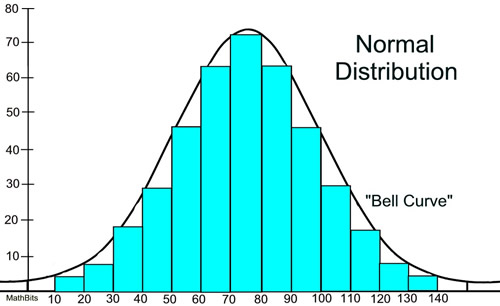
\includegraphics[width=.4\linewidth]{normal.png}
\caption{Distribuição de probabilidade contínua simétrica em ambos os lados da média.}
\label{fig:test}
\end{figure}
  
\section{Relação com outras disciplinas}

\par A cadeira ET586 - ESTATIST PROBABILIDADE COMPUTACAO é pré-requesito para a cadeira IF699 - APRENDIZAGEM DE MAQUINA, uma vez que é preciso entender alguns modelos estatístico antes de cursar essa cadeira.

\section{Referências}

Segue abaixo algumas referências usadas:

\par Estatística: 
\url{https://pt.wikipedia.org/wiki/Estat%C3%ADstica}

\par Probabilidade:
\url{https://pt.wikipedia.org/wiki/Probabilidade}

\par Machine Learning e a Estatística:
\url{https://bityli.com/JvIl0}






\end{document}
